%%%%%%%%%%%%%%%%%%%%%%%%%%%%%%%%%%%%%%%%%%%%%%%%%%%%%%%
% Please note that whilst this template provides a 
% preview of the typeset manuscript for submission, it 
% will not necessarily be the final publication layout.
%
% letterpaper/a4paper: US/UK paper size toggle
% num-refs/alpha-refs: numeric/author-year citation and bibliography toggle




%\documentclass[letterpaper]{oup-contemporary}
\documentclass[a4paper,num-refs]{oup-contemporary}

%%% Journal toggle; only specific options recognised.
%%% (Only "gigascience" and "general" are implemented now. Support for other journals is planned.)
\journal{general}

\usepackage{graphicx}
\usepackage{siunitx}
\usepackage{multirow}

%%% Flushend: You can add this package to automatically balance the final page, but if things go awry (e.g. section contents appearing out-of-order or entire blocks or paragraphs are coloured), remove it!
% \usepackage{flushend}

\title{Ultra-deep, long-read nanopore sequencing of mock microbial community standards}

%%% Use the \authfn to add symbols for additional footnotes, if any. 1 is reserved for correspondence emails; then continuing with 2 etc for contributions.
\author[1\authfn{2}]{Samuel M. Nicholls}
\author[1\authfn{2}]{Joshua C. Quick}
\author[2]{Shuiquan Tang}
\author[1\authfn{1}]{Nicholas J. Loman}

\affil[1]{Institute of Microbiology and Infection, School of Biosciences, University of Birmingham, UK}
\affil[2]{Zymo Research Corporation, Irvine, California, USA}

%%% Author Notes
\authnote{\authfn{1}n.j.loman@bham.ac.uk}
\authnote{\authfn{2}Contributed equally.}

%%% Paper category
\papercat{Data Note}

%%% "Short" author for running page header
\runningauthor{Nicholls and Quick et al.}

%%% Should only be set by an editor
\jvolume{00}
\jnumber{0}
\jyear{2018}

\begin{document}

\begin{frontmatter}
\maketitle
\begin{abstract}
\textbf{Background}: 
Long sequencing reads are information-rich: aiding \textit{de novo} assembly and reference mapping, and consequently have great potential for the study of microbial communities. However, the best approaches for analysis of long-read metagenomic data are unknown. Additionally, rigorous evaluation of bioinformatics tools is hindered by a lack of long-read data from validated samples with known composition.  \\
\textbf{Methods}: We sequenced two commercially-available mock communities containing ten microbial species (ZymoBIOMICS Microbial Community Standards) with Oxford Nanopore GridION and PromethION. Isolates from the same mock community were sequenced individually with Illumina HiSeq. \\
\textbf{Data}: We generated 14 and 16 Gbp from GridION flowcells and 146 and 148 Gbp from PromethION flowcells for the even and odd communities respectively. Read length N50 was 5.3 Kbp and 5.2 Kbp for the even and log community, respectively. Basecalls and corresponding signal data are made available (4.2 TB in total).
\\
\textbf{Results}: Alignment to Illumina-sequenced isolates demonstrated the expected microbial species at anticipated abundances, with the limit of detection for the lowest abundance species below 50 cells (GridION). \textit{De novo} assembly of metagenomes recovered long contiguous sequences without the need for pre-processing techniques such as binning.
\\
\textbf{Conclusions}: We present ultra-deep, long-read nanopore datasets from a well-defined mock community. These datasets will be useful for those developing bioinformatics methods for long-read metagenomics and for the validation and comparison of current laboratory and software pipelines. 

\end{abstract}
\begin{keywords}
bioinformatics; metagenomics; mock community; nanopore; single-molecule sequencing; real-time sequencing; benchmark; GridION; PromethION; Illumina; \textit{de novo} assembly
\end{keywords}
\end{frontmatter}

%%% Key points will be printed at top of second page
%\begin{keypoints*}
%\begin{itemize}
%\item This is the first point
%\item This is the second point
%\item One last point.
%\end{itemize}
%\end{keypoints*}

\section{Data Description}

Whole-genome sequencing of microbial communities (metagenomics) has revolutionised our view of microbial evolution and diversity, with numerous potential applications for microbial ecology, clinical microbiology and industrial biotechnology \cite{Handelsman2004-lg,Hug2016-wz}.
Typically, metagenomic studies use high-throughput sequencing platforms (\textit{e.g.} Illumina) \cite{Quince2017-lf} which generate very high yield, but of limited read length (100$-$300 bp).

In contrast, single-molecule sequencing platforms such as the Oxford Nanopore MinION, GridION and PromethION are able to sequence very long fragments of DNA (>10 Kbp, with over 2 Mbp reported) \cite{Jain2018-aw,Payne2018-cv} and with recent improvements to the platform making metagenomic studies using nanopore more viable, such studies are increasing in frequency \cite{Sanderson2018-zf,Charalampous2018-fl,Somerville2018-mq,Leggett2017-sx}. 
Long reads help with alignment-based assignment of taxonomy and function due to their increased information content \cite{Huson2007-mk,Wommack2008-qf}. 
Additionally, long reads permit bridging of repetitive sequences (within and between genomes), aiding genome completeness in \textit{de novo} assembly \cite{Bertrand2018-lz}.
However, these advantages are constrained by high error rate ($\approx$10\%), requiring the use of specific long-read alignment and assembly methods, which are either not specifically designed for metagenomics, or have not been extensively tested on real data \cite{sczyrba2017critical}.

Mock community standards are useful for the development of genomics methods \cite{Mason2017-yj}, and for the validation of existing laboratory, software and bioinformatics approaches. For example, validating the accuracy of a taxonomic identification pipeline is important, because the consequences of erroneous taxonomic identification from a metagenomic analysis may be severe, \textit{e.g.} in public health microbiology (such as in the well-publicised case of anthrax and plague in the New York Subway \cite{Ackelsberg2015-fh}) or missed diagnoses in the clinic. Mock community standards can also be used as positive controls during laboratory work, for example to validate that DNA extraction methods will yield expected representation of a sampled community \cite{Mason2017-yj}. 

Here, we present four nanopore sequencing datasets of two microbial community standards, providing a state-of-the-art benchmark to accelerate the development of methods for analysing long-read metagenomics data.

\begin{table*}[t!]
\centering
\caption{Description of the ten organisms comprising the ZymoBIOMICS Mock Community Standards.}
\label{tab:strains}
\begin{tabular}{r | l | l | l | l | l | c}
\toprule
 & & {Estimated Size} & NRRL & ATCC & Sequence & Illumina \\
 Species & Type & {(Mbp)} & Accession & Accession & Type &  FASTQ \\
\midrule
\textit{Bacillus subtilis}          & Gram $+$  & 4.045 & \texttt{B-354}   & \texttt{6633}& \texttt{ST7}   & \texttt{ERR2935851} \\
\textit{Cryptococcus neoformans}  & \multirow{2}{*}{Yeast} & \multirow{2}{*}{18.9} & \multirow{2}{*}{\texttt{Y-2534}}   & \multirow{2}{*}{$-$} & \multirow{2}{*}{$-$} & \multirow{2}{*}{\texttt{ERR2935856}} \\
$\times$ \textit{Cryptococcus deneoformans} & & & & & \\
\textit{Enterococcus faecalis}      & Gram $+$ & 2.845 & \texttt{B-537}   & \texttt{7080}& \texttt{ST55}  & \texttt{ERR2935850} \\
\textit{Escherichia coli}           & Gram $-$ & 4.875 & \texttt{B-1109}   & $-$& \texttt{ST10}  & \texttt{ERR2935852} \\
\textit{Lactobacillus fermentum}    & Gram $+$ & 1.905 & \texttt{B-1840}   & \texttt{14931}& $-$  & \texttt{ERR2935857} \\
\textit{Listeria monocytogenes}     & Gram $+$ & 2.992 & \texttt{B-33116}  & \texttt{19117}& \texttt{ST449}  & \texttt{ERR2935854} \\
\textit{Pseudomonas aeruginosa}     & Gram $-$ & 6.792 & \texttt{B-3509}   & \texttt{15442}& \texttt{ST252}  & \texttt{ERR2935853} \\
\textit{Saccharomyces cerevisiae}   & Yeast & 12.1 & \texttt{Y-567}    & \texttt{9763}& $-$  & \texttt{ERR2935855} \\
\textit{Salmonella enterica}        & Gram $-$ & 4.760 & \texttt{B-4212}    & $-$& \texttt{ST139} & \texttt{ERR2935848} \\
\textit{Staphylococcus aureus}      & Gram $+$ & 2.730 & \texttt{B-41012}  & $-$& \texttt{ST9}  & \texttt{ERR2935849} \\
\bottomrule
\end{tabular}
\begin{tablenotes}
\item Table adapted from ZymoBIOMICS™ Microbial Community Standard II (Log Distribution) Instruction Manual v1.1.2 Table 2 and Appendix A
\end{tablenotes}
\end{table*}

\begin{table*}[b!]
\centering
\caption{Summary of the four nanopore sequencing experiments.}\label{tab:datasets}
\begin{tabular}{l l | l l | c c S S | S S}
\toprule
     Signal &    FASTQ   		    &          &			   & {Time} & {Reads} & {N50} & {Quality} & {Yield} & {Q$>$7} \\
     Accession&Accession & Sequencer & Standard & {(h)} & {(M)} & {(Kbp)} & {(Median Q)} & {(Gbp)} & {(Gbp)} \\
\midrule
\texttt{ERR2887847} & \texttt{ERR2906227} & GridION &  Zymo CS Even \texttt{ZRC190633}  & 48 & 3.49	&  5.3 & 9.8	& 14.01 & 12.31 \\
\midrule
\texttt{ERR2887850} &\texttt{ERR2906229} & GridION &  Zymo CSII Log \texttt{ZRC190842}  	& 48 & 5.73	&  5.2 & 9.3	& 16.03 & 13.67 \\
\midrule
\texttt{ERR2887848} & \multirow{2}{*}{\texttt{ERR2906228}}& PromethION& Zymo CS Even \texttt{ZRC190633} & 64 &{\multirow{2}{*}{36.5}} & {\multirow{2}{*}{5.3}} & {\multirow{2}{*}{9.1}} & {\multirow{2}{*}{146.29}} & {\multirow{2}{*}{123.27}}\\
\texttt{ERR2887849} & & PromethION& Zymo CS Even \texttt{ZRC190633} & -- &  &    & &  \\
\midrule
\texttt{ERR2887851} & \multirow{2}{*}{\texttt{ERR2906230}} & PromethION& Zymo CSII Log \texttt{ZRC190842} 	&64& {\multirow{2}{*}{35.1}} & {\multirow{2}{*}{5.2}} & {\multirow{2}{*}{9.2}} & {\multirow{2}{*}{148.03}} & {\multirow{2}{*}{126.12}} \\
\texttt{ERR2887852} && PromethION& Zymo CSII Log \texttt{ZRC190842} 	&--&  &    & & \\


\bottomrule
\end{tabular}
\begin{tablenotes}
\item PromethION runs were restarted following the standard 64 hour protocol. The table reflects total yield across both the standard run and subsequent restarts.
\end{tablenotes}
\end{table*}

\subsection{Background Information}
The ZymoBIOMICS Microbial Community Standards (CS and CSII) are each composed of ten microbial species: eight bacteria and two yeasts (Table \ref{tab:strains}). The organisms in CS (hereafter referred to as `Even') are distributed equally (12\%), with the exception of the two yeasts which are each present at 2\%.
Cell counts from organisms in CSII (hereafter referred to as `Log') community are distributed on a log scale, with theoretical community composition ranging from 89.1\% (\textit{Listeria monocytogenes}), down to 0.000089\% (\textit{Staphylococcus aureus}).
%The standards are certified by the manufacturer to contain no more than 0.01\% contaminating cells.

\section{Methods}

\subsection{DNA extraction}

DNA was extracted from \SI{75}{\micro\litre} ZymoBIOMICS Microbial Community Standard (Product D6300, Lot ZRC190633) and \SI{375}{\micro\litre} ZymoBIOMICS Microbial Community Standard II (Product D6310, Lot ZRC190842) using the ZymoBIOMICS DNA Miniprep extraction kit according to manufacturer's instructions, with the following modifications to increase fragment length and maintain the expected representation of the Gram-negative species which are already lysed in the DNA/RNA Shield storage solution.
The standard was spun at 8,000$\times$\textit{g} for 5 minutes before removing the supernatant and retaining. The cell pellet was resuspended in \SI{750}{\micro\litre} lysis buffer and added to the ZR BashingBead lysis tube. Bead-beating was performed on a FastPrep-24 (MP Biomedicals) instrument for 2 cycles of 40 seconds with 5 minutes sitting on ice between cycles. The bead tubes were spun at 10,000$\times$\textit{g} for 1 minute and \SI{450}{\micro\litre} of supernatant was transferred to a Zymo Spin III-F filter before being spun again at 8000$\times$\textit{g} for 1 minute.
\SI{45}{\micro\litre} (Even) and \SI{225}{\micro\litre} (Log) of the supernatant retained earlier was combined with \SI{450}{\micro\litre} filtrate before adding \SI{1485}{\micro\litre} (Even) or \SI{2025}{\micro\litre} (Log) Binding Buffer and mixing before loading onto the column.

\subsection{Nanopore sequencing library preparation}

Quantification steps were performed using the dsDNA HS assay for Qubit. 
DNA was size-selected by cleaning up with 0.45$\times$ volume of Ampure XP (Beckman Coulter) and eluted in \SI{100}{\micro\litre} EB (Qiagen). Libraries were prepared from \SI{1400}{\nano\gram} input DNA using the LSK-109 kit (Oxford Nanopore Technologies) as per manufacturer's protocol, except incubation times for end-repair, dA-tailing and ligation were increased to 30 minutes to improve ligation efficiency. The even and log libraries were split and used on both the GridION and PromethION flowcells.

\subsection{Sequencing}

Sequencing libraries were quantified and two aliquots of \SI{50}{\nano\gram} and \SI{400}{\nano\gram} were prepared for GridION and PromethION sequencing respectively. The GridION sequencing was performed using a \texttt{FLO-MIN106} (rev.C) flowcell, \texttt{MinKNOW} 1.15.1 and standard 48-hour run script with active channel selection enabled. The PromethION sequencing was performed using a \texttt{FLO-PRO002} flowcell, \texttt{MinKNOW} 1.14.2 and standard 64-hour run script with active channel selection enabled.

Refuelling was performed approximately every 24h (GridION, PromethION) by loading \SI{75}{\micro\litre} (GridION) or \SI{150}{\micro\litre} (PromethION) refuelling mix (SQB diluted 1:2 with nuclease-free water). Additionally, after the standard scripts had completed the PromethION was restarted several times to utilise remaining active pores and maximise total yield.

\subsection{Nanopore basecalling}
Reads were basecalled on-instrument using the GPU basecaller \texttt{Guppy} (Oxford Nanopore Technologies) with the supplied \texttt{dna\_r9.4.1\_450bps\_prom.cfg} configuration (PromethION) and \texttt{dna\_r9.4\_450bps.cfg} (GridION). \texttt{Guppy} version 1.8.3 and 1.8.5 were installed on the GridION and PromethION respectively.

\subsection{Illumina sequencing}

DNA was extracted from pure cultures of each species using the ZymoBIOMICS DNA Miniprep Kit. Library preparation was performed using the Kapa HyperPlus Kit with \SI{100}{\nano\gram} DNA as input and TruSeq Y-adapters. The purified library derived from each sample was quantified by TapeStation (Agilent 4200) and pooled together in an equimolar fashion. The final library was sequenced on an Illumina HiSeq 1500 instrument using 2$\times$101 bp (paired-end) sequencing. Raw reads were demultiplexed using \texttt{bcl2fastq} v2.17.
%Shotgun sequencing of the even and log communities were performed with the same protocol.

%%%%%%%%%%%%%%%%%%%%%%%%%%%%%%%%%%%%%%%%
\begin{figure*}[t!] 
\centering
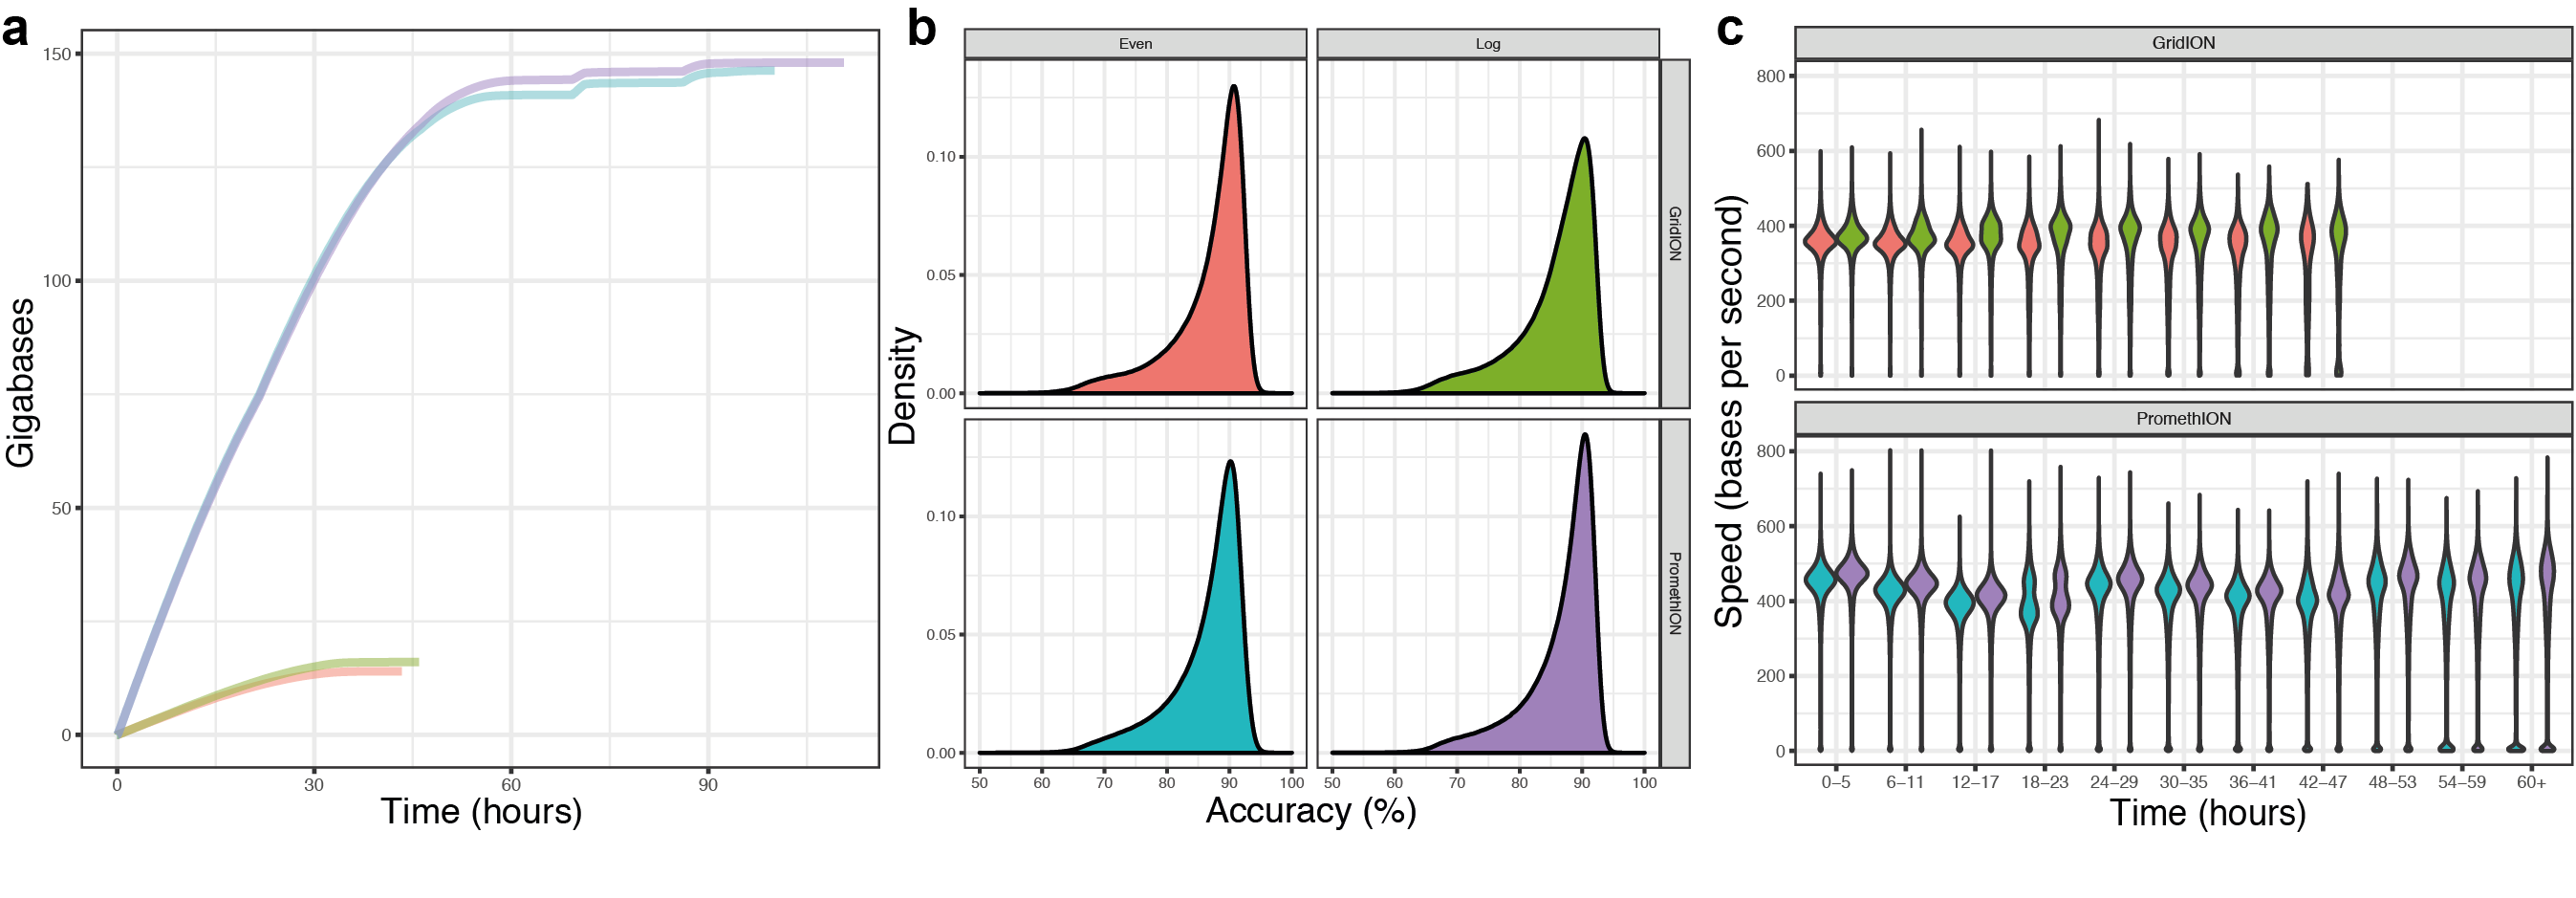
\includegraphics[width=0.995\linewidth]{figures/Figure1.png}
\caption{
Summary plots for the four generated data sets:
(a) collector's curve showing sequencing yield over time for each of the four sequencing runs,
(b) density plot showing sequence accuracy (\texttt{BLAST}-like identities),
(c) violin plot showing sequencing speed over time split by sequencing group.
}\label{fig:summaries}
\end{figure*}
\begin{figure}[b!]
\centering
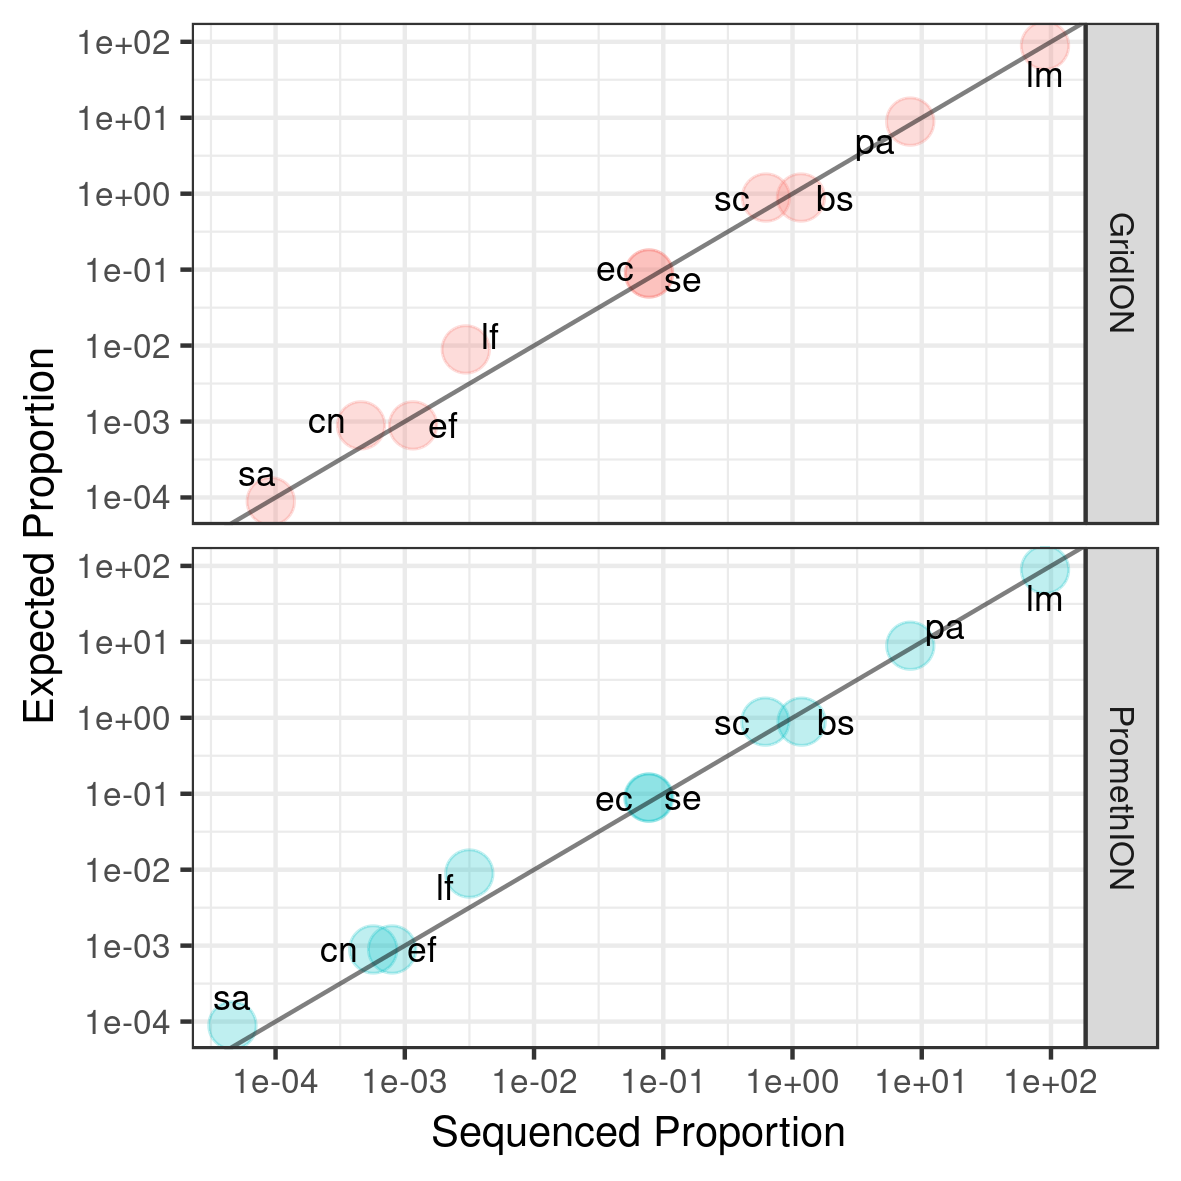
\includegraphics[width=\linewidth]{figures/log-ove.png}
\caption{Proportion of sequenced DNA from each of the 10 organisms that was sequenced (x-axis), against the proportion of yield expected given the known community composition (y-axis) of the Zymo CSII (Log) standard.}\label{fig:log-ove}
\end{figure}
%%%%%%%%%%%%%%%%%%%%%%%%%%%%%%%%%%%%%%%%%%%

\subsection{Bioinformatics}
To construct reference genomes, Illumina reads for each of the ten isolates were assembled using \texttt{SPAdes} v3.12.0 \cite{Bankevich2012-iu} with paired-end reads as input, using parameters \texttt{-m 512 -t 12}.
Scaffolds from \texttt{SPAdes} less than 500 bp length or with less than 10$\times$ coverage were removed. The remaining scaffolds were combined into a single mock community draft assembly for downstream analysis.

Nanopore reads were aligned to the mock community draft assembly using \texttt{minimap2} \cite{li2018minimap2} v2.14-r883 with parameters \texttt{-ax map-ont -t 12} and converted to a sorted BAM file using \texttt{samtools} \cite{li2009sequence}.
To reduce erroneous mappings, alignment BAM files were filtered using a script \texttt{bamstats.py} according to the following criteria; reference mapping length $\geq$500 bp, map quality (MAPQ) > 0, there are no supplementary alignments for this read and read is not a secondary alignment.
Coverage statistics were generated using the \texttt{summariseStats.R} Rscript. 


Read accuracy was determined by calculating \texttt{BLAST} identity from the filtered alignments (as per \url{http://lh3.github.io/2018/11/25/on-the-definition-of-sequence-identity}), calculated as $(L-NM)/L$ using the \texttt{minimap2} number of mismatches (\texttt{NM}) SAM tag and the sum of match, insertion and deletion CIGAR operations (\texttt{L}). 
\vfill\null

\begin{table*}[t!]
\caption{Read alignment statistics for even samples, showing absolute measurements and proportion of sequencing yield and the estimated genome coverage obtained for each organism in the mock community.}\label{tab:mappings-even}
\begin{tabularx}{\linewidth}{l c | S S c S | S S c S }
\toprule
{} & {} & \multicolumn{4}{c|}{GridION} & \multicolumn{4}{c}{PromethION} \\
{} & {Expected} & {Yield} & {Measured} & {Aln. N50} & {Coverage} & {Yield} & {Measured} & {Aln. N50} & {Coverage} \\
{Species} & {Proportion} & {(Gbp)} & {Proportion} & {(Kbp)} & {($\times$)} & {(Gbp)} & {Proportion} & {(Kbp)} & {($\times$)} \\
\midrule
\textit{Bacillus subtilis}			&12& 2.09 &19.30     &4.30& 516.41 	& 21.54 &18.98   &4.40&   5325.31	\\
\textit{Listeria monocytogenes} 	&12& 1.57 &14.53     &4.46& 525.44	& 16.20 &14.28   &4.57&   5414.09	\\
\textit{Enterococcus faecalis}		&12& 1.32 &12.21     &4.45& 464.33	& 13.66 &12.04   &4.56&   4802.85	\\
\textit{Staphylococcus aureus}		&12& 1.22 &11.25     &4.46& 445.98	& 12.58 &11.08   &4.57&   4607.07	\\
\textit{Salmonella enterica}		&12& 1.08 &10.01     &8.56& 227.50	& 11.76 &10.36   &8.94&   2470.85	\\
\textit{Escherichia coli}			&12& 1.08 &9.95     &8.31& 220.93	& 11.69 &10.30   &8.70&   2397.58	\\
\textit{Pseudomonas aeruginosa} 	&12& 1.05 &9.73     &9.00& 155.08	& 11.58 &10.20   &9.37&   1704.32	\\
\textit{Lactobacillus fermentum}	&12& 1.01 &9.30     &3.6& 528.46	& 10.35 &9.12   &3.72&   5433.40	\\
\textit{Saccharomyces cerevisiae} 	&2& 0.21  &1.92     &4.08& 17.18	& 2.12 	&1.87   &4.17&   174.97	\\
\textit{Cryptococcus neoformans}	&2& 0.19  &1.79     &4.44& 10.23	& 2.00	&1.76   &4.53&   105.95	\\
\bottomrule
\end{tabularx}
%\begin{tablenotes}
%\item
%\end{tablenotes}
\end{table*}
\begin{table*}[tb!]
\centering
\caption{Read alignment statistics for log samples, describing sequencing yield and estimated genome coverage obtained for each organism in the mock community.}\label{tab:mappings-odd}
\begin{tabular}{l | S c S | S c S }
\toprule
{} & \multicolumn{3}{c|}{GridION} & \multicolumn{3}{c}{PromethION} \\
{} & {Yield} & {Aln. N50} & {Coverage} & {Yield} & {Aln. N50} & {Coverage} \\
{Species} & {(Gbp)} & {(Kbp)} & {($\times$)} & {(Gbp)} & {(Kbp)} & {($\times$)} \\
\midrule
\textit{Listeria monocytogenes} 	& 11.85     &4.94& 3960.85   &  109.69  &4.97& 36659.72\\
\textit{Pseudomonas aeruginosa} 	& 1.08      &9.38& 158.83 &  10.06      &9.33& 1481.29\\
\textit{Bacillus subtilis}			& 0.15      &5.02& 37.89  & 1.44        &5.03& 355.39 \\
\textit{Saccharomyces cerevisiae} 	& 0.08      &4.76& 6.79   &  0.75       &4.74& 62.19\\
\textit{Salmonella enterica}		& 0.01      &9.26& 2.15   & 0.10        &9.14& 20.09 \\
\textit{Escherichia coli}			& 0.01      &8.72& 2.11   & 0.09        &9.17& 19.33 \\
\textit{Lactobacillus fermentum}	& 4E-4    &3.39& 0.207   & 0.004     &3.35& 2.03  \\
\textit{Enterococcus faecalis}		& 2E-4    &7.50& 0.086    & 1E-4    &6.81& 0.50 \\
\textit{Cryptococcus neoformans}	& 6E-5   &4.39& 0.003   &  7E-4    &4.96& 0.036\\
\textit{Staphylococcus aureus}		& 2E-5   &3.87& 0.006   & 8E-5    &3.03& 0.028 \\
\bottomrule
\end{tabular}
\begin{tablenotes}
\item Note that expected and measured proportions are illustrated by Figure \ref{fig:log-ove}.
\end{tablenotes}
\end{table*}

We used \texttt{wtdbg2} v2.2 to assemble nanopore data (\url{https://github.com/ruanjue/wtdbg2}).
\texttt{wtdbg2} was compiled from source in November 2018 from Git commit \texttt{094f2b3}. For GridION, all nanopore reads were used. For PromethION, we used both the full dataset and a random 25\% subsample. Subsampling was performed using (\texttt{subsample.py}).

Assemblies were conducted under a variety of parameter values for homopolymer-compressed k-mer size (\texttt{-p}), minimum graph edge weight support (\texttt{-e}) and read length threshold (\texttt{-L}). Global parameters for all runs (\texttt{-S1 -K10000 --node-max 6000}) were used to turn-off k-mer subsampling (to remove assembly stochasticity) and increase the coverage thresholds applied to k-mers and constructed nodes.

Assembly accuracy was determined by a modified version of \texttt{fastmer.py} (\url{https://github.com/jts/assembly\_accuracy}) which uses \texttt{minimap2} to align nanopore metagenomic contigs against the reference draft assembly.

\section{Results}

\subsection{Nanopore sequencing metrics}

We generated a total of 324.36 Gbp of sequence from the four nanopore sequencing runs (Table \ref{tab:datasets}, Figure \ref{fig:assemblies}.a).
PromethION flow cells generated approximately ten-times more sequencing data than the comparative GridION runs and showed equivalent read length N50 and quality scores (Figure \ref{fig:summaries}.b).
We observe a difference in sequencing speed between the PromethION (mean 395 bps and 412 bps for even and log) and the GridION (mean speed 341 and 359 bps for even and log) (Figure \ref{fig:summaries}.c).

\subsection{Illumina sequencing metrics}
%Dataset size for isolates, shotgun metagenomics and range of sizes for isolates, accession numbers.

Illumina datasets for the ten individually sequenced isolates averaged 13.53 million pairs of reads (ranging between 7.1 $-$ 23.2 million), with proportions of reads with a mean \texttt{phred} score $\geq$30 ranging between 75.51\% $-$ 93.09\% (mean 87.72\%).
ENA accession numbers for the isolates can be found in Table \ref{tab:strains}.

%The shotgun metagenomics sequencing of the even community generated 47.83 million read pairs, with an average \texttt{phred} score of 95.71\%.
%The shotgun metagenomics experiment can be downloaded from ENA with accession \texttt{ERR2935805}.


\begin{figure*}[t!]
\centering
\includegraphics[width=\linewidth]{figures/w2.png}
\caption{Bar plots demonstrating total length and contiguity of genomic assemblies obtained with \texttt{wtdbg2} from each of the long-read nanopore data sets. For each organism in the community (coloured columns), contigs longer than 10 kbp are horizontally stacked along the x-axis. Each row represents a run of \texttt{wtdbg2}, with the parameters for edge support, read length threshold and homopolymer-compressed k-mer size labelled on the left. Assemblies are grouped by the data set on which they were run (row facets). Additionally, assemblies may be compared to the estimated true genome size, and per-isolate Illumina \texttt{SPADES} assembly. Estimated genomes sizes are the same as those found in Table \ref{tab:strains}, however to display approximate chromosomes, the two yeasts were replaced by their corresponding canonical NCBI references for visualisation purposes only. The \textit{C. neoformans} strain used by the Zymo standards is a diploid genetic cross, which may explain the larger assemblies, compared to the represented estimated haploid size.
}\label{fig:assemblies}
\end{figure*}


\subsection{Nanopore mapping statistics}

We identify the presence of all 10 microbial species in the community, for both even and log samples, in expected proportions (Figure \ref{fig:log-ove}). For the even community, the GridION results provide sufficient depth (i.e. significantly >30$\times$ coverage) to potentially assemble all eight of the bacteria. The coverage of the yeast genomes were lower (10 and 17$\times$), potentially sufficient for assembly scaffolding. On the PromethION all genomes had >100$\times$ mean coverage (Tables \ref{tab:mappings-even} and \ref{tab:mappings-odd}).

For the log-distributed community, three taxa have sufficient coverage for assembly on GridION, compared with four on PromethION. On PromethION, a further two genomes (\textit{S. enterica} and \textit{E. coli}) have sufficient coverage for assembly scaffolding. We are able to detect \textit{S. aureus}, the lowest abundance organism on both platforms, with 32 reads from PromethION (from 450 cell input) and 7 reads from GridION (from 50 cell input).

\subsection{Nanopore metagenome assemblies}

We evaluated nanopore metagenomic assemblies and assessed genome completeness and contiguity for each run with different assembly parameters.

For the even community, genomes of the expected size were present for each of the bacterial species contained in small numbers of large contigs (Figure \ref{fig:assemblies}). However, the two yeasts are poorly represented in the assembly, consistent with their low read depth. 

\textit{L. monocytogenes} is poorly assembled in the log dataset despite being the most abundant organism, indicating very high sequence coverage may be detrimental to the performance of \texttt{wtdbg2}. We also observe that assembling the entire PromethION dataset resulted in less complete and more fragmented assemblies. This led us to sample randomly the PromethION data to 25\% of the total dataset which improved the assembly results.

After subsampling, assemblies of the even community from the GridION and PromethION are similar. However, the assemblies from PromethION data had better representation of the yeasts (particularly \textit{C. neoformans}), due to the higher coverage depths of these species.

Average consensus accuracy was calculated for the entire set of assemblies (n=51). For the even community, accuracy is 99.1\% ($\pm$ 0.17\%) and 99.0\% ($\pm$ 0.24\%) for the GridION and PromethION respectively. For the log community, average accuracy is 99.0\% ($\pm$ 0.27\%) and 99.1\% ($\pm$ 0.20\%) for the GridION and PromethION respectively.

\section{Discussion}

There are several noteworthy aspects of this dataset: We generated nearly 300 Gbp of sequence data from the Oxford Nanopore PromethION and 30 gigabases from the Oxford Nanopore GridION, on a well-characterised mock community sample and we have made basecalls and electrical signal data for each of the four runs presented here available: a combined dataset size of over four terabytes. The availability of the raw signal permits future basecalling of the data (an area under rapid development), as well as signal-level polishing and the detection of methylated bases \cite{Simpson2017-gn}.

Individual sequencing libraries were split between the GridION and PromethION, permitting direct comparisons of the instruments to be made. We observed high concordance between the datasets from each platform. We note the sequencing speed of the PromethION is faster than the GridION, which we attribute to different running temperatures on these instrument (39$^{\circ}$C versus 34$^{\circ}$C, respectively).

Confident detection of \textit{S. aureus} was demonstrated for the  GridION run to <50-cells using the log community. The PromethION generated around five times the number of \textit{S. aureus} reads as the GridION, but appears less sensitive as we loaded eight times more library. However, it may be possible to reduce the loading input to PromethION flowcells, but we have not attempted this.

Early results of metagenomics assembly show promise for reconstruction of whole microbial genomes from mixed samples without a binning step. We focused on the recently released \texttt{wtdbg2} software as we found that the established \texttt{minimap2} and \texttt{miniasm} method resulted in excessively large intermediate files (tens of terabases per analysis) which were impractical to store and analyse. 

For the even community, using \texttt{wtdgb2} with varying parameter choices, we were able to assemble seven of the bacteria into single contigs. However, no single parameter set was found to be optimum for both total genome size and contig length. 

We found that \texttt{wtdbg2} expects a maximum of 200$\times$ sample coverage, and discards sequence k-mers and \textit{de Bruijn} graph nodes with more than 200$\times$ support. These limits must be lifted by specifying higher \texttt{-K} and \texttt{--node-max} for this dataset. Increasing \texttt{-e} improved contiguity for the even sample, however this resulted in the loss of yeasts from the assembly. Increasing the read length threshold (\texttt{-L}) improved assembly contiguity for all sample and platform combinations, at the cost of genome size. Increasing the homopolymer-compressed k-mer size (\texttt{-p}) from the default of 21 to 23 also appears to improve assembly contiguity. It should be noted that \texttt{wtdbg2} is still under active development, making it difficult to make concrete recommendations for parameters.

The availability of this dataset should help with further improvements to long-read assembly techniques. Though, this study has several shortcomings:

We have not yet explored polishing techniques to improve consensus accuracy of assemblies using nanopore or Illumina data \cite{Rang2018-md}. A new ``flip-flop'' basecaller, \texttt{Flappie} (\url{https://github.com/nanoporetech/flappie}), was recently made available although we have not used it on this dataset.

Although reference genomes for the ten microbial strains contained in the standards are available from Zymo (\url{https://s3.amazonaws.com/zymo-files/BioPool/ZymoBIOMICS.STD.refseq.v2.zip}), they are constructed from a combination of nanopore and Illumina data (not presented here). To avoid a circular comparison, we chose to perform analysis only against Illumina draft genomes. 

Other mock microbial samples are available which we did not test here. The most notable alternative mock community sample is from the Human Microbiome Project (HMP) and consists of 20 microbial samples (available from BEI Resources). Nanopore metagenomic datasets for the HMP mock community have been sequenced as part of other studies, although the datasets are much smaller than the ones presented here \cite{Leggett2017-sx,Bertrand2018-lz,Huson2018-bh}.

\subsection{Re-use potential}
The provision of Illumina reads for each isolate permits a ground-truth to be obtained for the individual species contained in the mock community. This will be useful for training new nanopore basecalling and polishing models, long-read aligners, variant callers, and validating taxonomic assignment and assembly software and pipelines.

%\subsection{Citations and References}
%Use the \verb|num-refs| document class option for numerical citations, and \verb|alph-refs| option for author-year citations.
%Use the \verb|\citep| command for parenthetical citations, and \verb|\citet| command for text citations (when using \verb|alpha-refs|).


%\emph{GigaScience} encourages and assists with the submission of detailed protocols to the open access repository \href{https://www.protocols.io/}{protocols.io}. Please enter the details into protocols.io, issue a DOI, and cite the protocols.io record from the Methods section.

%Authors benefit greatly by posting their methods in protocols.io as these are in a formatted form, allow inclusion of all the details, are fully searchable unlike supplementary files, and can be updated to new versions as basic methodology changes over time. Doing this saves authors extensive time in the future as the methods do not need to be rewritten in future manuscripts as they need only be cited.

\section{Availability of source code and requirements}
Python and R scripts used to generate the summary information and analyses are open source and freely available via our repository (\url{https://github.com/LomanLab/mockcommunity}), under the MIT license.

%Lists the following:
%\begin{itemize}
%\item Project name: e.g.~My bioinformatics project
%\item Project home page: e.g.~\url{http://sourceforge.net/projects/mged}
%\item Operating system(s): e.g.~Platform independent
%\item Programming language: e.g.~Java
%\item Other requirements: e.g.~Java 1.3.1 or higher, Tomcat 4.0 or higher
%\item License: e.g.~GNU GPL, FreeBSD etc.
%Any restrictions to use by non-academics: e.g. licence needed
%\end{itemize}


\section{Availability of supporting data and materials}
%``The data set(s) supporting the results of this article is(are) available in the [repository name] repository, [cite unique persistent identifier].''
Unprocessed FASTQ from the Illumina sequencing of the ten isolates are available at the European Nucleotide Archive, via the identifiers listed in Table \ref{tab:strains}. 
Both the raw signal, and basecalled FASTQ for the Nanopore sequencing experiments are available at the European Nucleotide Archive, via the identifiers listed in Table \ref{tab:datasets}.
Further updates will be made available on our project website \url{https://lomanlab.github.io/mockcommunity/}.
This manuscript, and its supporting data are available under a Creative Commons Attribution 4.0 International (CC BY 4.0) license.

%Supplementary Python and R scripts used to conduct analyses are available in our Github repository: \url{https://github.com/LomanLab/mockcommunity}.

\vfill\null
\section{Declarations}

%\subsection{List of abbreviations}
%If abbreviations are used in the text they should be defined in the text at first use, and a list of abbreviations should be provided in alphabetical order.

%\subsection{Ethical Approval (optional)}
%Not applicable

\subsection{Consent for publication}
Not applicable

\subsection{Competing Interests}
Cambridge Biosciences provided the ZymoBIOMICS Microbial Community Standard free of charge.
ST is an employee of Zymo Research Corporation.
NJ has received Oxford Nanopore Technologies (ONT) reagents free of charge to support his research programme.
NJ and JQ have received travel expenses to speak at ONT events.
NL has received an honorarium to speak at an ONT company meeting.

\subsection{Funding}
SN is funded by the Medical Research Foundation and the NIHR STOP-COLITIS project.
JQ is funded by the NIHR Surgical Reconstruction and Microbiology Research Centre. 
The NIHR SRMRC is a partnership between The National Institute for Health Research, University Hospitals Birmingham NHS Foundation Trust, the University of Birmingham, and the Royal Centre for Defence Medicine.
NL is funded by an MRC Fellowship in Microbial Bioinformatics under the CLIMB project.

\subsection{Author's Contributions}
Conceptualization: NL, Methodology: NL JQ SN ST, Software: SN NL, Validation: SN NL, Formal analysis: SN NL, Investigation: NL JQ SN, Resources: NL ST, Data Curation: SN NL ST, Writing – original draft preparation: SN, Writing – review and editing: SN NL JQ ST, Visualization: SN NL, Supervision: NL, Project administration: NL, Funding acquisition: NL ST

%The individual contributions of authors to the manuscript should be specified in this section. Guidance and criteria for authorship can be found in our \href{https://academic.oup.com/gigascience/pages/editorial_policies_and_reporting_standards}{editorial policies}. We would recommend you follow some kind of standardised taxonomy like the \href{http://docs.casrai.org/CRediT}{CASRAI CRediT} (Contributor Roles Taxonomy).


\section{Acknowledgements}

We are grateful to Radoslaw Poplawski (University of Birmingham) for assistance with CLIMB virtual machines and file systems to support this research. We thank Divya Mirrington (Oxford Nanopore Technologies) for advice on PromethION library preparation and sequencing. We thank Hannah McDonnell at Cambridge Biosciences for providing the ZymoBIOMICS Microbial Community Standards. We thank Jared Simpson (Ontario Institute for Cancer Research), Matt Loose (University of Nottingham) and John Tyson (University of British Columbia) for useful discussions and advice.

%\section{Authors' information (optional)}
%You may choose to use this section to include any relevant information about the author(s) that may aid the reader's interpretation of the article, and understand the standpoint of the author(s). This may include details about the authors' qualifications, current positions they hold at institutions or societies, or any other relevant background information. Please refer to authors using their initials. Note this section should not be used to describe any competing interests.



%% Specify your .bib file name here, without the extension
\bibliography{paper-refs}



\end{document}
